%% ProcessMusic.tex
%% V0.1
%% 2012/10/23
%% by Kyle Kastner
%%
%% requires IEEEtran.cls version 1.7 or later
%% This file based on content from http://www.ctan.org/tex-archive/macros/latex/contrib/IEEEtran/

\documentclass[journal]{IEEEtran}
\usepackage[labelfont=bf]{caption}
\captionsetup[figure]{labelformat=parens}
\usepackage{graphicx}
\usepackage{amsmath}
\usepackage{flushend}
\newcommand\numberthis{\addtocounter{equation}{1}\tag{\theequation}}
\begin{document}
\title{A Saga of Pet Recognition, using the Asirra Dataset 
       and Deep Convolutional Neural Networks}

\author{Kyle Kastner\\University of Texas-San Antonio}

\maketitle

\begin{abstract}
Deep learning is the broad term for the recent development and extensions 
of neural networks in the machine learning community, which has allowed for
state of the art results in speech, image, and natural language processing
tasks. This paper will explore a deep neural network architecture for
classifying objects in images for the CIFAR10 and Asirra dataset. 
This research focuses on a two class image recognition 
problem, which is made up of images featuring cats and
dogs in various sizes, colors, positions, and locations. Experimentation has
shown that advanced preprocessing can be extremely helpful in solving this 
problem, and some recent research on transfer learning (learning from other
data) has yielded a very powerful, simple new preprocessing technique.
\end{abstract}
% IEEEtran.cls defaults to using nonbold math in the Abstract.
% This preserves the distinction between vectors and scalars. However,
% if the journal you are submitting to favors bold math in the abstract,
% then you can use LaTeX's standard command \boldmath at the very start
% of the abstract to achieve this. Many IEEE journals frown on math
% in the abstract anyway.

% Note that keywords are not normally used for peerreview papers.
\begin{IEEEkeywords}
Convolutional neural network, ZCA, dropout, maxout, CIFAR10, Asirra, 
transfer learnin, image processing, machine learning 
\end{IEEEkeywords}

\IEEEpeerreviewmaketitle
\section{Introduction}
\IEEEPARstart{N}{eural} networks have a rich history in the A.I. and machine
learning communities, starting with the perceptron algorithm in 1957 
\cite{Perceptron}. The perceptron algorithm is considered by many as the 
direct precursor to modern neural networks, though effective computation of the
neural network was not achieved until 1975 with the invention of the 
backpropagation algorithm \cite{Backprop}. Most recently, neural networks have
returned in several A.I. related fields: "machine learning", "big data", and 
"data analytics" among them. The massive volumes of data available for modern 
research, coupled with algorithmic improvements and massively increased 
computing power, have allowed the once purely theoretical "neural network" to
achieve state of the art results in real world image, speech, and 
text processing tasks. Outpacing more traditional feature oriented techniques 
in each respective field, neural networks are a topic of interest in both 
academia and industry. As the focus turns away from algorithms and towards 
"big data", it is important to remember that good data, with good
preprocessing, can allow even very simple algorithms to support incredible
performance on many problems. In this paper, logistic regression, 
support vector machines, and deep neural networks coupled with a convolutional
preprocessing feature (called DeCAF \cite{DeCAF}) will be put to the test.

\section{Dataset}
The datasets used for these experiments were the CIFAR10 dataset \cite{CIFAR10}
and the Asirra dataset \cite{Asirra}, both of which are comprised of 3 channel
RGB  images, and a single label which describes the contents of the image.
CIFAR10 images are 32x32 pixels by default, and the Asirra images were modified
to fit the structure of the ImageNet dataset, which was required for the 
convolutional feature generation. ImageNet images are large by default with
center cropping done on a 224x224 
pixel region. The Asirra images were rescaled to 224x224 for this experiment,
in order to approximately match the scale of ImageNet.
The ImageNet dataset features 1200000 images representing 
one thousand different classes of objects, and is used for many different 
computer vision challenges every year. Though this dataset was not directly
used for this testing, it was used to create the convolutional preprocessing 
architecture that was used as preprocessing. The CIFAR10 dataset features 60000 
images representing ten different classes of objects, as listed below.
\begin{itemize}
\item automobile
\item airplane
\item bird 
\item cat
\item deer
\item dog
\item frog
\item horse
\item ship
\item truck
\end{itemize}
The Asirra dataset used for these experiments features 25000 images, containing
objects representing the classes listed below.
\begin{itemize}
\item cat
\item dog
\end{itemize}

\section{Preprocessing}
The key preprocessing step taken for both of these datasets was to apply zero
phase component analysis (ZCA) to each training set. Mathematically, this 
technique can be described by Eq. \ref{eq:ZCA} \cite{CIFAR10}. By centering 
new data (subtracting the column-wise mean of $X$), and applying $W$ as shown in 
Eq. \ref{eq:whiten}, the whitened result $X_w$ is obtained. This ZCA 
whitened result has been shown to resemble the effects of the human vision
system \cite{ZCA}, and improves classification results in the CIFAR10 task 
by a wide margin \cite{CIFAR10}. It is crucial that the $W$ matrix obtained 
during the training phase is applied to the test set, rather than calculating
a new $W$ using the test data.
\begin{equation}
W = (XX^T)^{\frac{1}{2}} = ED^{\frac{1}{2}}E^T
\label{eq:ZCA}
\end{equation}
\begin{equation}
X_w = XW
\label{eq:whiten}
\end{equation}


ZCA, coupled with global contrast normalization (GCN) is a near requirement for 
image processing with neural networks. However, the recent publication of the 
DeCAF network \cite{DeCAF} has significantly altered the landscape, and
provides a large improvement over other methods. DeCAF is both a deep neural
network and a non-linear preprocessing scheme - it is a full convolutional 
network, trained on the \emph{entire} ImageNet dataset \cite{TorontoImageNet}.
Once this network has been learned the bottom 6 layers are frozen and used as
non-linear preprocessing, with an output vector or 4096. This output can then 
be used as the feature input to more standard machine learning algorithms.The
authors of the DeCAF paper have published their trained network weights, which
means this can be treated as a "black box" feature extractor for images. A 
secondary benefit is that the \emph{application} of this neural network is not
computationally intensive, which means the final algorithm chosen for
discrimination will be the dominant processing cost.

\section{Network Architecture}
Neural networks for image processing often utilize a special layer called a
convolutional layer for the first few stages \cite{Convolutional}, in order 
to capture the spatial relationships between pixels and colors, as shown in 
Fig. \ref{fig:convolutional}. This allows for a more effective representation
of the image during the learning phase, and also allows for some interesting
visualizations of the layer one filters. This will be explored more extensively
in the next section.

\begin{figure}[h!]
\centering
  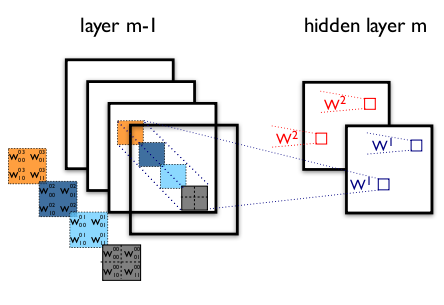
\includegraphics[width=0.45\textwidth]{convolutional.png}
  \caption{Convolutional layer visualization \cite{LeNetTut}}
\label{fig:convolutional}
\end{figure}

Another technique used in this architecture is a maxout layer, which is a new
"universal approximator" layer built specifically to take advantage of dropout
\cite{Dropout}. Using maxout units in place of rectified linear units typically
provides fair improvement in existing dropout networks \cite{Maxout}. 

\begin{figure}[h!]
\centering
  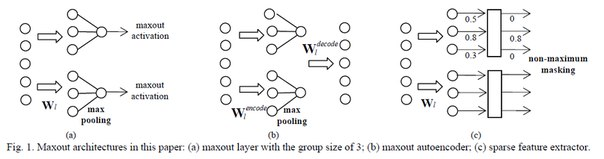
\includegraphics[width=0.45\textwidth]{maxout.png}
  \caption{Maxout layer visualization \cite{Lowresource}}
\label{fig:maxout}
\end{figure}

The overall network architecture and hyperparameter choices for the CIFAR10 
tests were chosen from a draft version of \cite{Maxout}. The authors have 
subsequently released a higher performing configuration, which requires more
computational resources. A nearly identical network and hyperparameters were 
chosen for the Asirra tests, with the main modification being that the Asirra
results used a fused training set of both the CIFAR10 data and the Asirra data,
in the hopes that the Asirra data would give discriminative power between cats
and dogs, while the CIFAR10 data would provide a baseline image recognition 
capability. This idea is very similar to the concept of the recently developed
DeCAF image processing technique \cite{DeCAF}. A summary of the hyperparameter
choices are shown below.

\begin{itemize}
\item Layer sizes: 48 - 128 - 128 - 240 - 10
\item Layer types: Convolutional (C) - C - C - Maxout - Softmax
\item Initial learning rate .1, decay .01 per epoch for 250 epochs
\item Initial momentum .5, ramping to .6 over 250 epochs
\item Stochastic gradient descent, batch size 128 
\item Dropout .8, scale 1 for layer 1, each layer after has dropout .5, scale 2
\item Weights initialized between (-.005, .005), random uniform distribution
\item Kernel shape, pool shape, pool stride for layer 1: (8, 8), (4, 4), (2, 2) 
\item Kernel shape, pool shape, pool stride for layer 2: (8, 8), (4, 4), (2, 2) 
\item Kernel shape, pool shape, pool stride for layer 3: (5, 5), (2, 2), (2, 2) 
\item Maxout group size: 5 
\end{itemize}

Further testing, using DeCAF for feature extraction, used the following 
algorithms and parameters.

\begin{itemize}
\item Logistic Regression 
\item Linear SVM 
\item Polynomial SVM, degree=3 
\item Deep neural network classifier 
\end{itemize}

The deep neural network featured the following parameters:
\begin{itemize}
\item Layer sizes: 5000 - 5000 - 5000 - 5000 - 2
\item Layer types: RectLinear(RL) - RL - RL - RL
\item Initial learning rate .01, decay .001 per epoch for 250 epochs
\item Initial momentum .5, ramping to .9 over 250 epochs
\item Stochastic gradient descent, batch size 128 
\item Dropout .8, scale 1 for layer 1, each layer after has dropout .5, scale 2
\item Sparse initialization of 15 random weight units 
\end{itemize}

\section{Results}
After training, the CIFAR10 network slightly exceeds the published state of the
art for unmodified training data, scoring 86.25\% on the test set. In Fig. 
\ref{fig:cifartrain}, the training and validation error are shown decreasing
over time, and the learned first layer filters are shown in Fig. 
\ref{fig:cifarweights}.

\begin{figure}[h!]
\centering
  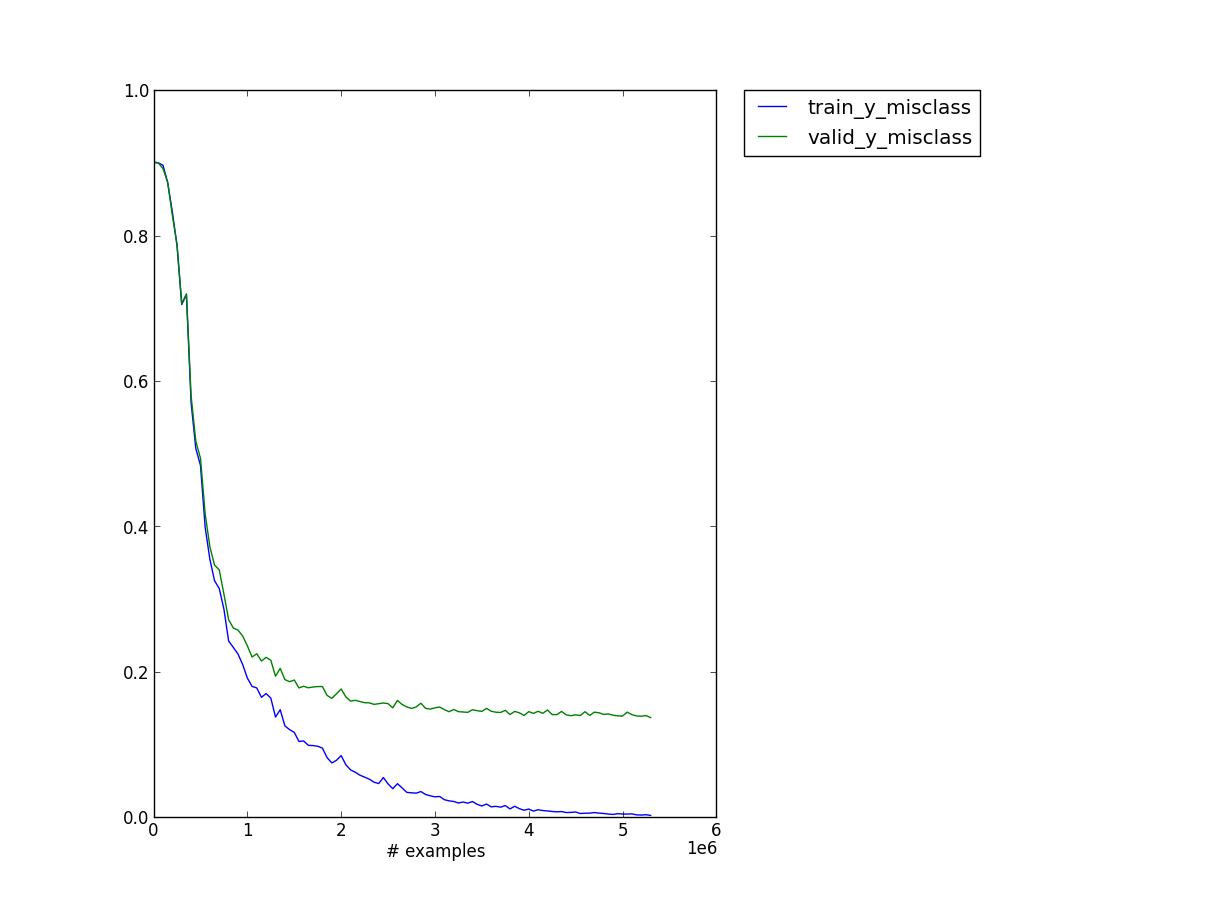
\includegraphics[width=0.45\textwidth]{cifartrain.png}
  \caption{CIFAR10 error}
\label{fig:cifartrain}
\end{figure}

\begin{figure}[h!]
\centering
  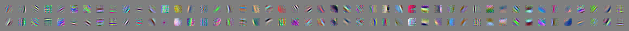
\includegraphics[width=0.45\textwidth]{cifarweights.png}
  \caption{CIFAR10 first layer filters}
\label{fig:cifarweights}
\end{figure}

Adding contrast normalization and random image flipping along the horizontal
(p=.5) gave a bump to the CIFAR10 result, scoring 88.9\% on the test set. 

\begin{figure}[h!]
\centering
  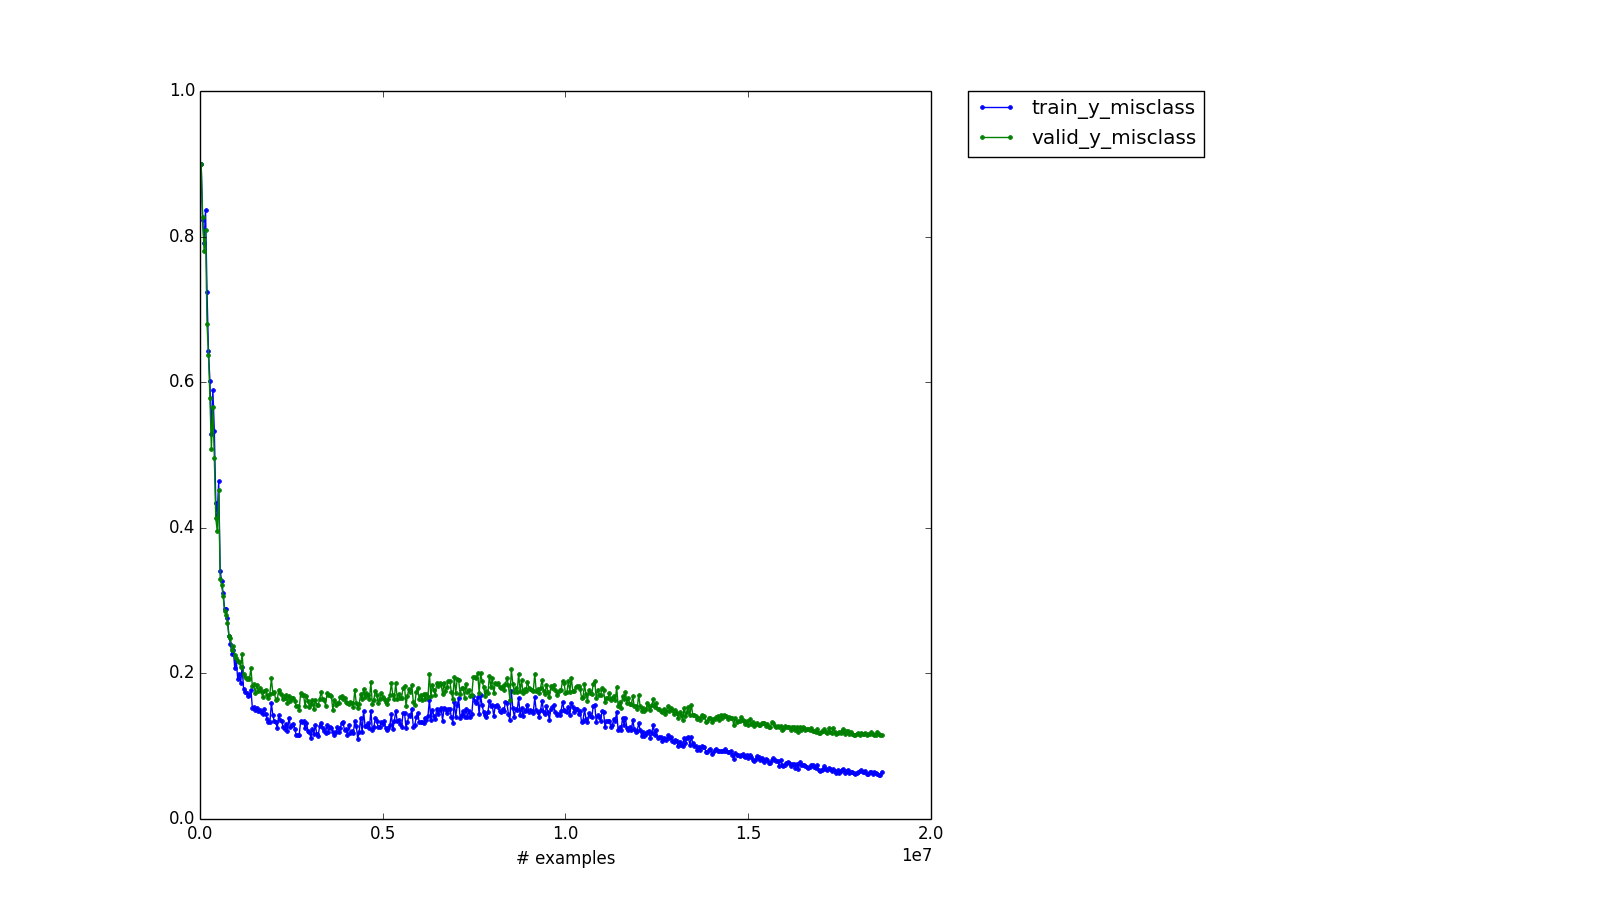
\includegraphics[width=0.45\textwidth]{cifar10.png}
  \caption{Improved CIFAR10 network \cite{Lowresource}}
\label{fig:cifar10}
\end{figure}

The next attempt was to use this same technique, using the Asirra data in 
conjuntion with the cats and dogs images present in CIFAR10.
The network trained on Asirra and CIFAR10 data combined seems to have very 
similar results to the network trained on only CIFAR10 data. In fact, it 
appears the mixing of the two datasets has let the CIFAR10 training dominate
the Asirra results, which means the data mixing experiment is largely a 
failure. This is likely due to excess shrinkage or distortion of the Asirra 
images in the conversion to 32x32 .png files from much larger .jpg files.
The results of this experiment are shown in Figs. \ref{fig:asirratrain} and 
\ref{figs:asirraweights}.

\begin{figure}[h!]
\centering
  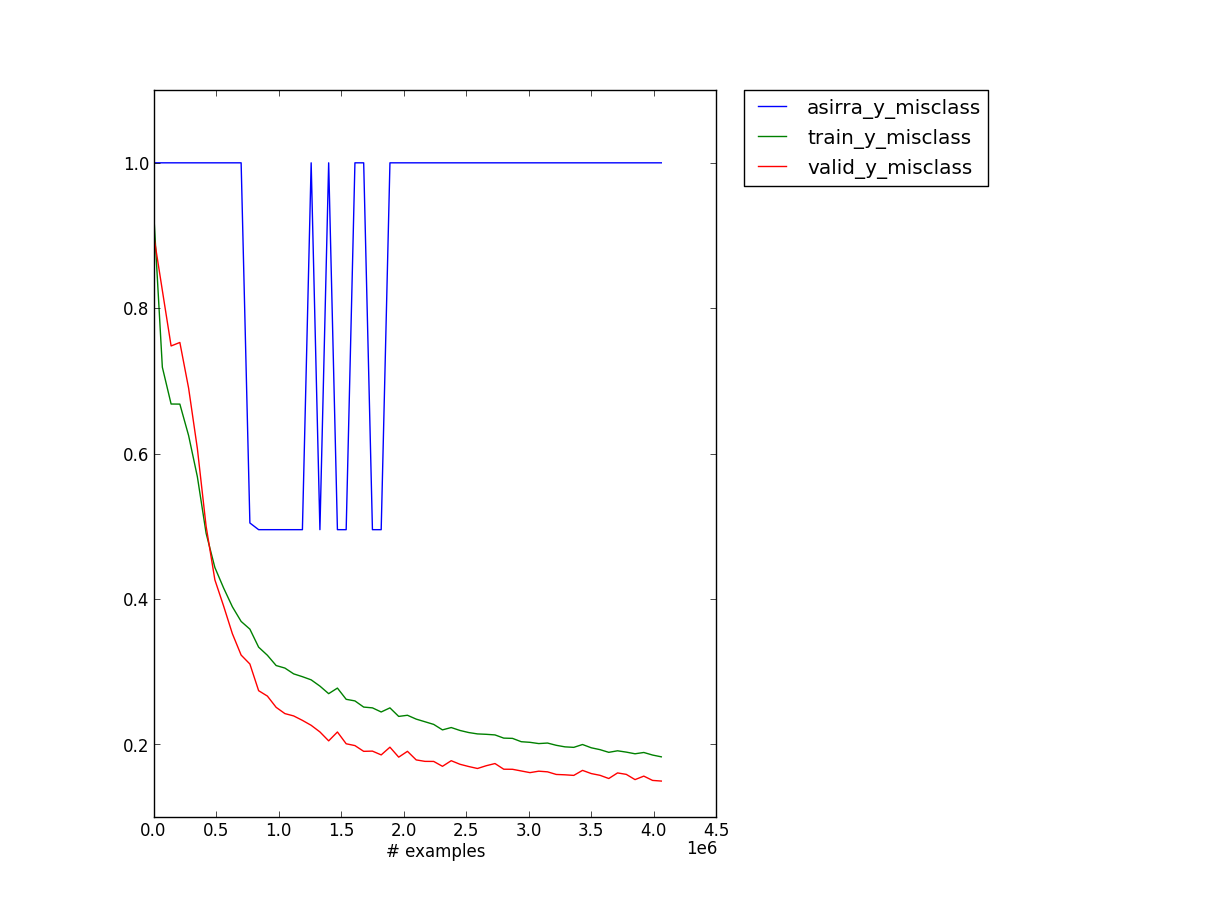
\includegraphics[width=0.45\textwidth]{asirratrain.png}
  \caption{Asirra + CIFAR10 error}
\label{fig:asirratrain}
\end{figure}

\begin{figure}[h!]
\centering
  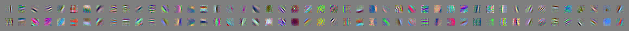
\includegraphics[width=0.45\textwidth]{asirraweights.png}
  \caption{Asirra + CIFAR10 first layer filters}
\label{fig:asirraweights}
\end{figure}

With these experiments running into difficulty, the DeCAF network for
preprocessing was put into the pipeline, in place of the other preprocessing 
techniques. This resulted in excellent results for all tested algorithms.

\begin{tabular}{l*{6}{c}r}
    Algorithm         & Validation Set Accuracy(\%) \\
    \hline
    Logistic Reg.     & 94   \\
    Linear SVM        & 94.2 \\
    Polynomial SVM(3) & 96   \\
    4-Layer NN        & 96.7 \\
\end{tabular}

\begin{figure}[h!]
\centering
  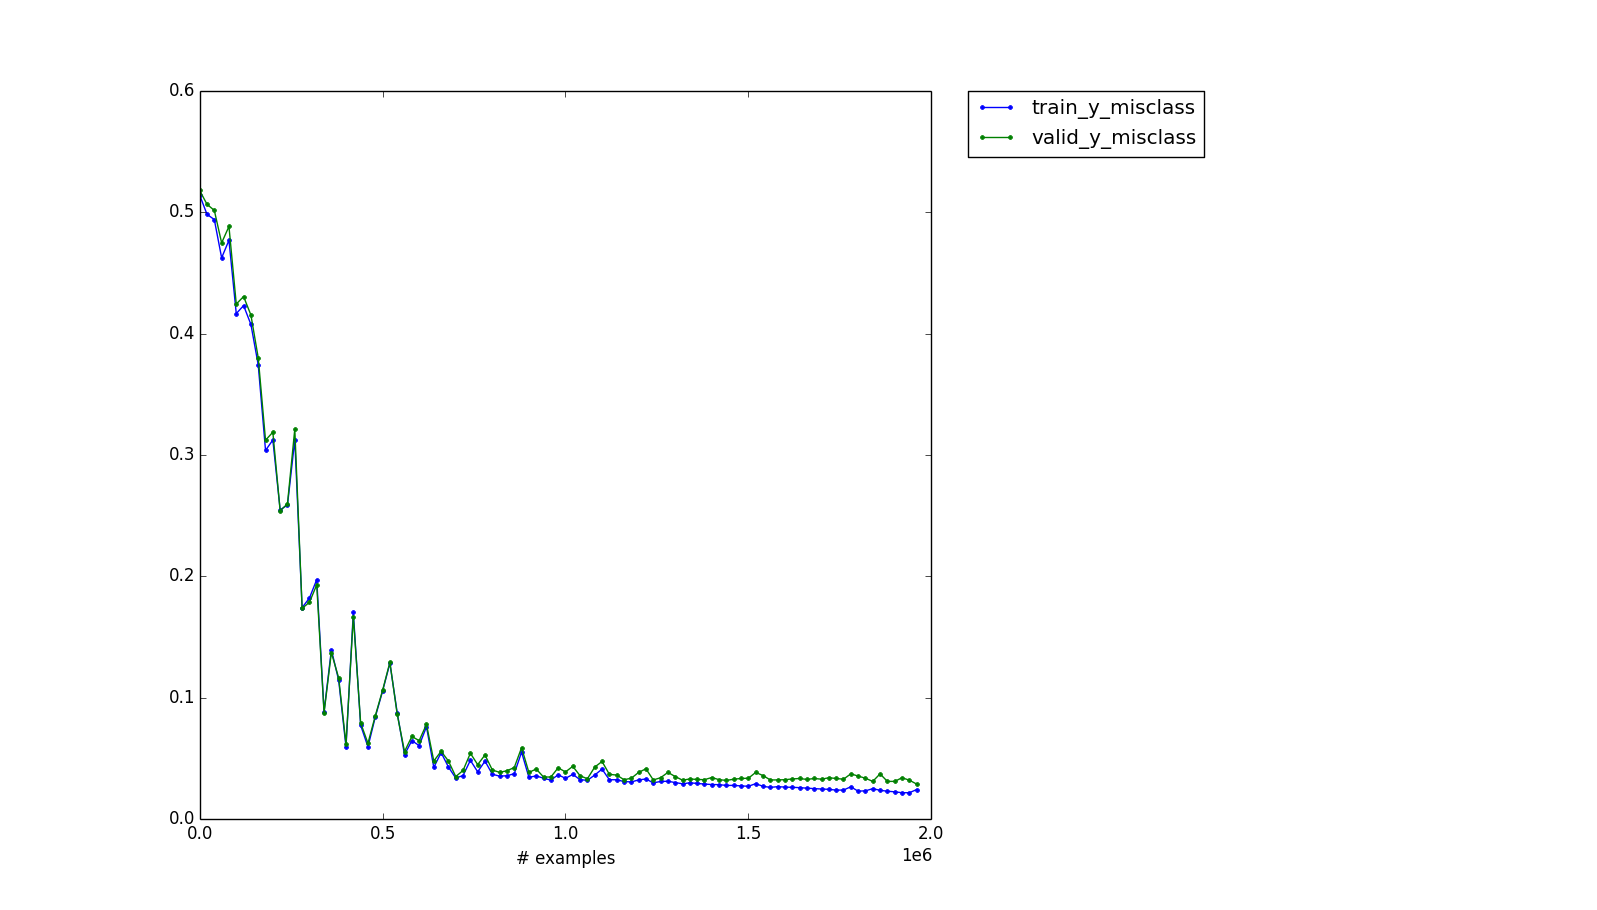
\includegraphics[width=0.45\textwidth]{asirra.png}
  \caption{Training error for Asirra dataset, deep classifier}
\label{fig:asirra}
\end{figure}
These results speak for themselves. Effectively, the DeCAF preprocessing allows
the simpler algorithms (SVM, logistic regression) to make decisions in a space
very similar to a neural network, without the training overhead. A further
comparison of "full network" training versus top layer only will be needed, but
requires full access to the ImageNet dataset.

\section{Conclusions}
The applicability of deep convolutional networks for image processing 
has been well established in both academic literature and industry, with this 
paper providing further backing. Using a deep convolutional network for the 
CIFAR10 dataset allows for recognition of objects in these images without 
feature engineering. This strongly hints that the convolutional network is able
to learn effective hierarchical representations of complex data, at least 
in this particular case. The results of \cite{Maxout} have also been repeated 
and verified, confirming the improvement provided by maxout layers in dropout
networks for image recognition. Unfortunately, the neural network trained on
a mix of Asirra and CIFAR10 data did not appear to provide any additional 
discriminative power for recognition of cats and dogs in the Asirra dataset. 
Much improvement was seen by switching to an already trained network which 
utilized a much broader dataset during training.
Preprocessing has always been a key part of building a solid machine learning 
pipeline, but the addition of DeCAF and other "deep" preprocessors is very
radical. The ability to get powerful results, with simple algorithms and 
advanced neural network based preprocessing is a very ingenious idea.
This idea has strong implications for robotics and vehicles, where the
complicated preprocessing could be "hard wired" into an FPGA or ASIC, 
thus allowing a computationally light algorithm on the back end to achieve
acceptable performance for embedded or battery critical applications.This 
result also resonates in other fields - if this representation can be 
learned for images, what about audio or video? So far, there is nothing to
suggest that this result is unique to images, and there are many research
avenues to explore.

\begin{thebibliography}{1}
\bibitem{Perceptron}
Rosenblatt F., \emph{The perceptron, a perceiving and recognizing automaton}. 
Report 85-460-1, Cornell Aeronautical Laboratory, 1957.
\bibitem{Backprop}
Werbos P.J., \emph{Beyond Regression: New Tools for Prediction and Analysis 
in the Behavioral Sciences}, 1975.
\bibitem{CIFAR10}
Krizhevsky A., \emph{Learning Multiple Layers of Features from Tiny Images},
2009. Retrieved from http://www.cs.toronto.edu/~kriz/cifar.html, 2013.
\bibitem{Asirra}
Elson J., Douceur J.R., Howell  J., Saul J., \emph{Asirra: A CAPTCHA 
that Exploits Interest-Aligned Manual Image Categorization}, in 
Proceedings of 14th ACM Conference on Computer and Communications Security 
(CCS), Association for Computing Machinery, Inc., Oct. 2007.
Subset retrieved from http://www.kaggle.com/c/dogs-vs-cats. 
\bibitem{ZCA}
Bell A.J., Sejnowski T.J., \emph{The "Independent Components" of Natural Scenes
are Edge Filters}, 37(23): 3327-3338, Vision Research, 1997.
\bibitem{Convolutional}
LeCun Y., Bengio Y., \emph{Convolutional Networks for Images, Speech, 
and Time-Series}, The Handbook of Brain Theory and Neural Networks, MIT Press, 
1995.
\bibitem{LeNetTut}
LISA Lab, University of Montreal, \emph{LeNet Tutorials}. Retrieved from 
http://deeplearning.net/tutorial/lenet.html, 2013.
\bibitem{Maxout}
Goodfellow I., Warde-Farley D., Mirza M., Courville A., Bengio Y., 
\emph{Maxout Networks}, JMLR WCP 28 (3): 1321-1327, 2013.
\bibitem{DeCAF}
Donahue J., Jia Y., Vinyals O., Hoffman J., Zhang N., Tzeng E., Darrell T., 
\emph{DeCAF: A Deep Convolutional Activation Feature for Generic 
Visual Recognition}, arXiv 1310.1531, 2013.
\bibitem{Lowresource}
Y. Miao, Metze F., S. Rawat \emph{Deep Maxout Networks for Low-Resource Speech Recognition}, in 
Proceeding of ASRU, Dec. 2013.
\bibitem{Dropout}
Hinton G., Srivastava N., Krizhevsky A., Sutskever I., Salakhutdinhov R., 
\emph{Improving neural networks by preventing co-adaptation of feature
detectors}, arXiv 1207.0580, 2012.
\bibitem{ImageNet}
Deng J., \emph{ImageNet: A Large Scale Hierarchical Image Database},
in Proceedings of The IEEE Conference on Computer Vision and Pattern 
Recognition (CVPR), Jun. 2009. pp. 248-255.
\bibitem{TorontoImageNet}
Krizhevsky A., Sutskever I. and Hinton G. E.
\emph{ImageNet Classification with Deep Convolutional Neural Networks}
NIPS 2012: Neural Information Processing Systems.
\end{thebibliography}

% You can push biographies down or up by placing
% a \vfill before or after them. The appropriate
% use of \vfill depends on what kind of text is
% on the last page and whether or not the columns
% are being equalized.

%\vfill

% Can be used to pull up biographies so that the bottom of the last one
% is flush with the other column.

\enlargethispage{-5in}
% that's all folks
\end{document}


